
 % Default to the notebook output style
 
     
 
 
 % Inherit from the specified cell style.
 
 
 
 
     
 \documentclass[11pt]{article}
 
     
     
     \usepackage[T1]{fontenc}
     % Nicer default font than Computer Modern for most use cases
     \usepackage{palatino}
 
     % Basic figure setup, for now with no caption control since it's done
     % automatically by Pandoc (which extracts ![](path) syntax from Markdown).
     \usepackage{graphicx}
     % We will generate all images so they have a width \maxwidth. This means
     % that they will get their normal width if they fit onto the page, but
     % are scaled down if they would overflow the margins.
     \makeatletter
     \def\maxwidth{\ifdim\Gin@nat@width>\linewidth\linewidth
     \else\Gin@nat@width\fi}
     \makeatother
     \let\Oldincludegraphics\includegraphics
     % Set max figure width to be 80% of text width, for now hardcoded.
     \renewcommand{\includegraphics}[1]{\Oldincludegraphics[width=.8\maxwidth]{#1}}
     % Ensure that by default, figures have no caption (until we provide a
     % proper Figure object with a Caption API and a way to capture that
     % in the conversion process - todo).
     \usepackage{caption}
     \DeclareCaptionLabelFormat{nolabel}{}
     \captionsetup{labelformat=nolabel}
 
     \usepackage{adjustbox} % Used to constrain images to a maximum size 
     \usepackage{xcolor} % Allow colors to be defined
     \usepackage{enumerate} % Needed for markdown enumerations to work
     \usepackage{geometry} % Used to adjust the document margins
     \usepackage{amsmath} % Equations
     \usepackage{amssymb} % Equations
     \usepackage{textcomp} % defines textquotesingle
     % Hack from http://tex.stackexchange.com/a/47451/13684:
     \AtBeginDocument{%
         \def\PYZsq{\textquotesingle}% Upright quotes in Pygmentized code
     }
     \usepackage{upquote} % Upright quotes for verbatim code
     \usepackage{eurosym} % defines \euro
     \usepackage[mathletters]{ucs} % Extended unicode (utf-8) support
     \usepackage[utf8x]{inputenc} % Allow utf-8 characters in the tex document
     \usepackage{fancyvrb} % verbatim replacement that allows latex
     \usepackage{grffile} % extends the file name processing of package graphics 
                          % to support a larger range 
     % The hyperref package gives us a pdf with properly built
     % internal navigation ('pdf bookmarks' for the table of contents,
     % internal cross-reference links, web links for URLs, etc.)
     \usepackage{hyperref}
 \usepackage{booktabs}
    \usepackage{longtable} % longtable support required by pandoc >1.10
     \usepackage{booktabs}  % table support for pandoc > 1.12.2
     \usepackage[normalem]{ulem} % ulem is needed to support strikethroughs (\sout)
                                 % normalem makes italics be italics, not underlines
     
 
     
     
     % Colors for the hyperref package
     \definecolor{urlcolor}{rgb}{0,.145,.698}
     \definecolor{linkcolor}{rgb}{.71,0.21,0.01}
     \definecolor{citecolor}{rgb}{.12,.54,.11}
 
     % ANSI colors
     \definecolor{ansi-black}{HTML}{3E424D}
     \definecolor{ansi-black-intense}{HTML}{282C36}
     \definecolor{ansi-red}{HTML}{E75C58}
     \definecolor{ansi-red-intense}{HTML}{B22B31}
     \definecolor{ansi-green}{HTML}{00A250}
     \definecolor{ansi-green-intense}{HTML}{007427}
     \definecolor{ansi-yellow}{HTML}{DDB62B}
     \definecolor{ansi-yellow-intense}{HTML}{B27D12}
     \definecolor{ansi-blue}{HTML}{208FFB}
     \definecolor{ansi-blue-intense}{HTML}{0065CA}
     \definecolor{ansi-magenta}{HTML}{D160C4}
     \definecolor{ansi-magenta-intense}{HTML}{A03196}
     \definecolor{ansi-cyan}{HTML}{60C6C8}
     \definecolor{ansi-cyan-intense}{HTML}{258F8F}
     \definecolor{ansi-white}{HTML}{C5C1B4}
     \definecolor{ansi-white-intense}{HTML}{A1A6B2}
 
     % commands and environments needed by pandoc snippets
     % extracted from the output of `pandoc -s`
     \providecommand{\tightlist}{%
       \setlength{\itemsep}{0pt}\setlength{\parskip}{0pt}}
     \DefineVerbatimEnvironment{Highlighting}{Verbatim}{commandchars=\\\{\}}
     % Add ',fontsize=\small' for more characters per line
     \newenvironment{Shaded}{}{}
     \newcommand{\KeywordTok}[1]{\textcolor[rgb]{0.00,0.44,0.13}{\textbf{{#1}}}}
     \newcommand{\DataTypeTok}[1]{\textcolor[rgb]{0.56,0.13,0.00}{{#1}}}
     \newcommand{\DecValTok}[1]{\textcolor[rgb]{0.25,0.63,0.44}{{#1}}}
     \newcommand{\BaseNTok}[1]{\textcolor[rgb]{0.25,0.63,0.44}{{#1}}}
     \newcommand{\FloatTok}[1]{\textcolor[rgb]{0.25,0.63,0.44}{{#1}}}
     \newcommand{\CharTok}[1]{\textcolor[rgb]{0.25,0.44,0.63}{{#1}}}
     \newcommand{\StringTok}[1]{\textcolor[rgb]{0.25,0.44,0.63}{{#1}}}
     \newcommand{\CommentTok}[1]{\textcolor[rgb]{0.38,0.63,0.69}{\textit{{#1}}}}
     \newcommand{\OtherTok}[1]{\textcolor[rgb]{0.00,0.44,0.13}{{#1}}}
     \newcommand{\AlertTok}[1]{\textcolor[rgb]{1.00,0.00,0.00}{\textbf{{#1}}}}
     \newcommand{\FunctionTok}[1]{\textcolor[rgb]{0.02,0.16,0.49}{{#1}}}
     \newcommand{\RegionMarkerTok}[1]{{#1}}
     \newcommand{\ErrorTok}[1]{\textcolor[rgb]{1.00,0.00,0.00}{\textbf{{#1}}}}
     \newcommand{\NormalTok}[1]{{#1}}
     
     % Additional commands for more recent versions of Pandoc
     \newcommand{\ConstantTok}[1]{\textcolor[rgb]{0.53,0.00,0.00}{{#1}}}
     \newcommand{\SpecialCharTok}[1]{\textcolor[rgb]{0.25,0.44,0.63}{{#1}}}
     \newcommand{\VerbatimStringTok}[1]{\textcolor[rgb]{0.25,0.44,0.63}{{#1}}}
     \newcommand{\SpecialStringTok}[1]{\textcolor[rgb]{0.73,0.40,0.53}{{#1}}}
     \newcommand{\ImportTok}[1]{{#1}}
     \newcommand{\DocumentationTok}[1]{\textcolor[rgb]{0.73,0.13,0.13}{\textit{{#1}}}}
     \newcommand{\AnnotationTok}[1]{\textcolor[rgb]{0.38,0.63,0.69}{\textbf{\textit{{#1}}}}}
     \newcommand{\CommentVarTok}[1]{\textcolor[rgb]{0.38,0.63,0.69}{\textbf{\textit{{#1}}}}}
     \newcommand{\VariableTok}[1]{\textcolor[rgb]{0.10,0.09,0.49}{{#1}}}
     \newcommand{\ControlFlowTok}[1]{\textcolor[rgb]{0.00,0.44,0.13}{\textbf{{#1}}}}
     \newcommand{\OperatorTok}[1]{\textcolor[rgb]{0.40,0.40,0.40}{{#1}}}
     \newcommand{\BuiltInTok}[1]{{#1}}
     \newcommand{\ExtensionTok}[1]{{#1}}
     \newcommand{\PreprocessorTok}[1]{\textcolor[rgb]{0.74,0.48,0.00}{{#1}}}
     \newcommand{\AttributeTok}[1]{\textcolor[rgb]{0.49,0.56,0.16}{{#1}}}
     \newcommand{\InformationTok}[1]{\textcolor[rgb]{0.38,0.63,0.69}{\textbf{\textit{{#1}}}}}
     \newcommand{\WarningTok}[1]{\textcolor[rgb]{0.38,0.63,0.69}{\textbf{\textit{{#1}}}}}
     
     
     % Define a nice break command that doesn't care if a line doesn't already
     % exist.
     \def\br{\hspace*{\fill} \\* }
     % Math Jax compatability definitions
     \def\gt{>}
     \def\lt{<}
     % Document parameters
     \title{L13StrongInductionInvariants}
     
     
     
 
     % Pygments definitions
     
 \makeatletter
 \def\PY@reset{\let\PY@it=\relax \let\PY@bf=\relax%
     \let\PY@ul=\relax \let\PY@tc=\relax%
     \let\PY@bc=\relax \let\PY@ff=\relax}
 \def\PY@tok#1{\csname PY@tok@#1\endcsname}
 \def\PY@toks#1+{\ifx\relax#1\empty\else%
     \PY@tok{#1}\expandafter\PY@toks\fi}
 \def\PY@do#1{\PY@bc{\PY@tc{\PY@ul{%
     \PY@it{\PY@bf{\PY@ff{#1}}}}}}}
 \def\PY#1#2{\PY@reset\PY@toks#1+\relax+\PY@do{#2}}
 
 \expandafter\def\csname PY@tok@nl\endcsname{\def\PY@tc##1{\textcolor[rgb]{0.63,0.63,0.00}{##1}}}
 \expandafter\def\csname PY@tok@nf\endcsname{\def\PY@tc##1{\textcolor[rgb]{0.00,0.00,1.00}{##1}}}
 \expandafter\def\csname PY@tok@ss\endcsname{\def\PY@tc##1{\textcolor[rgb]{0.10,0.09,0.49}{##1}}}
 \expandafter\def\csname PY@tok@s\endcsname{\def\PY@tc##1{\textcolor[rgb]{0.73,0.13,0.13}{##1}}}
 \expandafter\def\csname PY@tok@kp\endcsname{\def\PY@tc##1{\textcolor[rgb]{0.00,0.50,0.00}{##1}}}
 \expandafter\def\csname PY@tok@gt\endcsname{\def\PY@tc##1{\textcolor[rgb]{0.00,0.27,0.87}{##1}}}
 \expandafter\def\csname PY@tok@o\endcsname{\def\PY@tc##1{\textcolor[rgb]{0.40,0.40,0.40}{##1}}}
 \expandafter\def\csname PY@tok@err\endcsname{\def\PY@bc##1{\setlength{\fboxsep}{0pt}\fcolorbox[rgb]{1.00,0.00,0.00}{1,1,1}{\strut ##1}}}
 \expandafter\def\csname PY@tok@m\endcsname{\def\PY@tc##1{\textcolor[rgb]{0.40,0.40,0.40}{##1}}}
 \expandafter\def\csname PY@tok@gd\endcsname{\def\PY@tc##1{\textcolor[rgb]{0.63,0.00,0.00}{##1}}}
 \expandafter\def\csname PY@tok@bp\endcsname{\def\PY@tc##1{\textcolor[rgb]{0.00,0.50,0.00}{##1}}}
 \expandafter\def\csname PY@tok@cs\endcsname{\let\PY@it=\textit\def\PY@tc##1{\textcolor[rgb]{0.25,0.50,0.50}{##1}}}
 \expandafter\def\csname PY@tok@gh\endcsname{\let\PY@bf=\textbf\def\PY@tc##1{\textcolor[rgb]{0.00,0.00,0.50}{##1}}}
 \expandafter\def\csname PY@tok@c1\endcsname{\let\PY@it=\textit\def\PY@tc##1{\textcolor[rgb]{0.25,0.50,0.50}{##1}}}
 \expandafter\def\csname PY@tok@kt\endcsname{\def\PY@tc##1{\textcolor[rgb]{0.69,0.00,0.25}{##1}}}
 \expandafter\def\csname PY@tok@mf\endcsname{\def\PY@tc##1{\textcolor[rgb]{0.40,0.40,0.40}{##1}}}
 \expandafter\def\csname PY@tok@go\endcsname{\def\PY@tc##1{\textcolor[rgb]{0.53,0.53,0.53}{##1}}}
 \expandafter\def\csname PY@tok@gi\endcsname{\def\PY@tc##1{\textcolor[rgb]{0.00,0.63,0.00}{##1}}}
 \expandafter\def\csname PY@tok@ni\endcsname{\let\PY@bf=\textbf\def\PY@tc##1{\textcolor[rgb]{0.60,0.60,0.60}{##1}}}
 \expandafter\def\csname PY@tok@ow\endcsname{\let\PY@bf=\textbf\def\PY@tc##1{\textcolor[rgb]{0.67,0.13,1.00}{##1}}}
 \expandafter\def\csname PY@tok@vg\endcsname{\def\PY@tc##1{\textcolor[rgb]{0.10,0.09,0.49}{##1}}}
 \expandafter\def\csname PY@tok@gr\endcsname{\def\PY@tc##1{\textcolor[rgb]{1.00,0.00,0.00}{##1}}}
 \expandafter\def\csname PY@tok@ne\endcsname{\let\PY@bf=\textbf\def\PY@tc##1{\textcolor[rgb]{0.82,0.25,0.23}{##1}}}
 \expandafter\def\csname PY@tok@kn\endcsname{\let\PY@bf=\textbf\def\PY@tc##1{\textcolor[rgb]{0.00,0.50,0.00}{##1}}}
 \expandafter\def\csname PY@tok@w\endcsname{\def\PY@tc##1{\textcolor[rgb]{0.73,0.73,0.73}{##1}}}
 \expandafter\def\csname PY@tok@nt\endcsname{\let\PY@bf=\textbf\def\PY@tc##1{\textcolor[rgb]{0.00,0.50,0.00}{##1}}}
 \expandafter\def\csname PY@tok@gs\endcsname{\let\PY@bf=\textbf}
 \expandafter\def\csname PY@tok@kr\endcsname{\let\PY@bf=\textbf\def\PY@tc##1{\textcolor[rgb]{0.00,0.50,0.00}{##1}}}
 \expandafter\def\csname PY@tok@nd\endcsname{\def\PY@tc##1{\textcolor[rgb]{0.67,0.13,1.00}{##1}}}
 \expandafter\def\csname PY@tok@sb\endcsname{\def\PY@tc##1{\textcolor[rgb]{0.73,0.13,0.13}{##1}}}
 \expandafter\def\csname PY@tok@cp\endcsname{\def\PY@tc##1{\textcolor[rgb]{0.74,0.48,0.00}{##1}}}
 \expandafter\def\csname PY@tok@mi\endcsname{\def\PY@tc##1{\textcolor[rgb]{0.40,0.40,0.40}{##1}}}
 \expandafter\def\csname PY@tok@il\endcsname{\def\PY@tc##1{\textcolor[rgb]{0.40,0.40,0.40}{##1}}}
 \expandafter\def\csname PY@tok@gp\endcsname{\let\PY@bf=\textbf\def\PY@tc##1{\textcolor[rgb]{0.00,0.00,0.50}{##1}}}
 \expandafter\def\csname PY@tok@nn\endcsname{\let\PY@bf=\textbf\def\PY@tc##1{\textcolor[rgb]{0.00,0.00,1.00}{##1}}}
 \expandafter\def\csname PY@tok@ch\endcsname{\let\PY@it=\textit\def\PY@tc##1{\textcolor[rgb]{0.25,0.50,0.50}{##1}}}
 \expandafter\def\csname PY@tok@cm\endcsname{\let\PY@it=\textit\def\PY@tc##1{\textcolor[rgb]{0.25,0.50,0.50}{##1}}}
 \expandafter\def\csname PY@tok@ge\endcsname{\let\PY@it=\textit}
 \expandafter\def\csname PY@tok@se\endcsname{\let\PY@bf=\textbf\def\PY@tc##1{\textcolor[rgb]{0.73,0.40,0.13}{##1}}}
 \expandafter\def\csname PY@tok@sx\endcsname{\def\PY@tc##1{\textcolor[rgb]{0.00,0.50,0.00}{##1}}}
 \expandafter\def\csname PY@tok@k\endcsname{\let\PY@bf=\textbf\def\PY@tc##1{\textcolor[rgb]{0.00,0.50,0.00}{##1}}}
 \expandafter\def\csname PY@tok@sd\endcsname{\let\PY@it=\textit\def\PY@tc##1{\textcolor[rgb]{0.73,0.13,0.13}{##1}}}
 \expandafter\def\csname PY@tok@na\endcsname{\def\PY@tc##1{\textcolor[rgb]{0.49,0.56,0.16}{##1}}}
 \expandafter\def\csname PY@tok@mb\endcsname{\def\PY@tc##1{\textcolor[rgb]{0.40,0.40,0.40}{##1}}}
 \expandafter\def\csname PY@tok@kd\endcsname{\let\PY@bf=\textbf\def\PY@tc##1{\textcolor[rgb]{0.00,0.50,0.00}{##1}}}
 \expandafter\def\csname PY@tok@vi\endcsname{\def\PY@tc##1{\textcolor[rgb]{0.10,0.09,0.49}{##1}}}
 \expandafter\def\csname PY@tok@sc\endcsname{\def\PY@tc##1{\textcolor[rgb]{0.73,0.13,0.13}{##1}}}
 \expandafter\def\csname PY@tok@s2\endcsname{\def\PY@tc##1{\textcolor[rgb]{0.73,0.13,0.13}{##1}}}
 \expandafter\def\csname PY@tok@nc\endcsname{\let\PY@bf=\textbf\def\PY@tc##1{\textcolor[rgb]{0.00,0.00,1.00}{##1}}}
 \expandafter\def\csname PY@tok@mo\endcsname{\def\PY@tc##1{\textcolor[rgb]{0.40,0.40,0.40}{##1}}}
 \expandafter\def\csname PY@tok@gu\endcsname{\let\PY@bf=\textbf\def\PY@tc##1{\textcolor[rgb]{0.50,0.00,0.50}{##1}}}
 \expandafter\def\csname PY@tok@nb\endcsname{\def\PY@tc##1{\textcolor[rgb]{0.00,0.50,0.00}{##1}}}
 \expandafter\def\csname PY@tok@no\endcsname{\def\PY@tc##1{\textcolor[rgb]{0.53,0.00,0.00}{##1}}}
 \expandafter\def\csname PY@tok@mh\endcsname{\def\PY@tc##1{\textcolor[rgb]{0.40,0.40,0.40}{##1}}}
 \expandafter\def\csname PY@tok@sh\endcsname{\def\PY@tc##1{\textcolor[rgb]{0.73,0.13,0.13}{##1}}}
 \expandafter\def\csname PY@tok@sr\endcsname{\def\PY@tc##1{\textcolor[rgb]{0.73,0.40,0.53}{##1}}}
 \expandafter\def\csname PY@tok@nv\endcsname{\def\PY@tc##1{\textcolor[rgb]{0.10,0.09,0.49}{##1}}}
 \expandafter\def\csname PY@tok@s1\endcsname{\def\PY@tc##1{\textcolor[rgb]{0.73,0.13,0.13}{##1}}}
 \expandafter\def\csname PY@tok@si\endcsname{\let\PY@bf=\textbf\def\PY@tc##1{\textcolor[rgb]{0.73,0.40,0.53}{##1}}}
 \expandafter\def\csname PY@tok@cpf\endcsname{\let\PY@it=\textit\def\PY@tc##1{\textcolor[rgb]{0.25,0.50,0.50}{##1}}}
 \expandafter\def\csname PY@tok@c\endcsname{\let\PY@it=\textit\def\PY@tc##1{\textcolor[rgb]{0.25,0.50,0.50}{##1}}}
 \expandafter\def\csname PY@tok@kc\endcsname{\let\PY@bf=\textbf\def\PY@tc##1{\textcolor[rgb]{0.00,0.50,0.00}{##1}}}
 \expandafter\def\csname PY@tok@vc\endcsname{\def\PY@tc##1{\textcolor[rgb]{0.10,0.09,0.49}{##1}}}
 
 \def\PYZbs{\char`\\}
 \def\PYZus{\char`\_}
 \def\PYZob{\char`\{}
 \def\PYZcb{\char`\}}
 \def\PYZca{\char`\^}
 \def\PYZam{\char`\&}
 \def\PYZlt{\char`\<}
 \def\PYZgt{\char`\>}
 \def\PYZsh{\char`\#}
 \def\PYZpc{\char`\%}
 \def\PYZdl{\char`\$}
 \def\PYZhy{\char`\-}
 \def\PYZsq{\char`\'}
 \def\PYZdq{\char`\"}
 \def\PYZti{\char`\~}
 % for compatibility with earlier versions
 \def\PYZat{@}
 \def\PYZlb{[}
 \def\PYZrb{]}
 \makeatother
 
 
     % Exact colors from NB
     \definecolor{incolor}{rgb}{0.0, 0.0, 0.5}
     \definecolor{outcolor}{rgb}{0.545, 0.0, 0.0}
 
 
 
     
     % Prevent overflowing lines due to hard-to-break entities
     \sloppy 
     % Setup hyperref package
     \hypersetup{
       breaklinks=true,  % so long urls are correctly broken across lines
       colorlinks=true,
       urlcolor=urlcolor,
       linkcolor=linkcolor,
       citecolor=citecolor,
       }
     % Slightly bigger margins than the latex defaults
     
     \geometry{verbose,tmargin=1in,bmargin=1in,lmargin=1in,rmargin=1in}
     
     
 
     \begin{document}
     
     
 \DeclareGraphicsRule{.jpe}{jpg}{*}{}
    \maketitle
     
     
 
     
     \section{Lecture 13: Strong Induction and
 Invariants}\label{lecture-13-strong-induction-and-invariants}
 
     \subsection{Midterm 2 Special Office Hours and Updated
 Schedule}\label{midterm-2-special-office-hours-and-updated-schedule}
 
 \begin{itemize}
 \item
   Midterm 2 is on Tuesday during class time. Specific
   \href{https://lorecchia.github.io/CS131-Combinatoric-Structures/midterm2info.html}{info
   on course webpage}.
 \item
   \textbf{Special Office Hours}. In the Undegraduate Lab, unless
   specified otherwise:
 
   \begin{itemize}
   \tightlist
   \item
     \emph{Friday}: Jiadong 2-3.30pm; Hannah 3.30pm-5pm.\\
   \item
     \emph{Monday}: Lorenzo 12-1pm in Lorenzo's office, Sarah 2-4pm.\\
   \item
     \emph{Tuesday}: Hannah 11-12.30pm.
   \end{itemize}
 \item
   There will be no office hours nor labs on Tuesday night or Wednesday
   after the midterm.
 \item
   Grades will be available by Thursday morning. If you are considering
   dropping the class based on your grade, you may come and pick up your
   exam on Thursday morning.
 \end{itemize}
 
     \subsection{Recap of Previous
 Lectures}\label{recap-of-previous-lectures}
 
 \begin{itemize}
 \tightlist
 \item
   Principle of Mathematical Induction:
 \end{itemize}
 
 \begin{figure}
 \centering
 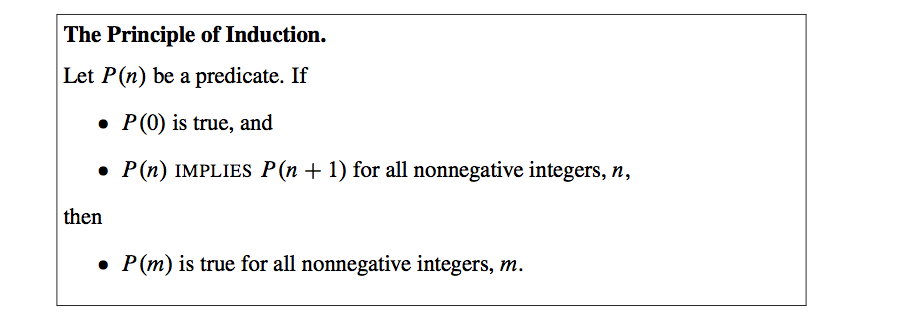
\includegraphics{images/L13/pmi.png}
 \caption{PMI}
 \end{figure}
 
     \begin{itemize}
 \tightlist
 \item
   Simple proofs by induction:
 
   \begin{itemize}
   \tightlist
   \item
     Arithmetic and Geometric Series
   \item
     Simple Inequalities
   \end{itemize}
 \end{itemize}
 
     \begin{itemize}
 \tightlist
 \item
   More advanced proofs by induction:
 
   \begin{itemize}
   \tightlist
   \item
     Geometric Proofs
   \end{itemize}
 \end{itemize}
 
     \begin{itemize}
 \tightlist
 \item
   Equivalence between Principle of Mathematical Induction and
   Well-Ordering Principle
 \end{itemize}
 
     \subsection{Importance of Choosing a Strong Inductive
 Hypothesis}\label{importance-of-choosing-a-strong-inductive-hypothesis}
 
 \textbf{Example}: Prove the following fundamental theorem.
 
 \begin{theorem}
 Every integer greater than $1$ is a product of primes.
 \end{theorem}
 
     \textbf{Question}: What should we make the inductive hypothesis \(P(n)\)
 be?
 
     \textbf{Answer}: Natural choice for \(n \geq 2\):
 
 \begin{itemize}
 \item P(n)  : $n$ _is a product of primes_
 
 \item Inductive step: $\forall n, P(n) \implies P(n+1)$
 
 <center>
 for all $n$, if $n$ is a product of primes then $n+1$ is a product of primes.
 </center>        
 \end{itemize}
 
     \textbf{Problem}: This seems hard. \(P(n)\) tells us very little about
 \(P(n+1)\).
 
     \textbf{Idea}: Change inductive hypothesis
 
     \subsection{Question: Change the Inductive
 Hypothesis}\label{question-change-the-inductive-hypothesis}
 
 \begin{theorem}
 Every integer greater than $1$ is a product of primes.
 \end{theorem}
 
 Let us use the same notation:\\
 
 \(P(n)\): \(n\) is a product of primes.
 
 \textbf{Idea}: Pick a different inductive hypothesis \(Q(n)\).
 
     \textbf{Question}: Which inductive hypothesis \(Q(n)\) is best suited to
 prove the theorem?
 
 \begin{itemize}
 \item for $n \geq 3,$  
 $Q(n): P(n) \land P(n-1)$
 
 \item for $n \geq 3,$    
 $Q(n): P(n) \land P(2) \land (n \;\textrm{odd} \implies P\left(\frac{n+1}{2}\right))$
 
 \item for $n \geq 2,$  
 $Q(n): \forall k \leq n, P(k)$
 
 \item for $n \geq 2,$  
 $Q(n): P(n) \land P(2)$
 \end{itemize}
 
     \textbf{Answer}: \(Q(n): \forall k \leq n, P(k)\)
 
 \textbf{Why does it help}: we can assume that \(P(k)\) has been proved
 for all \(k \leq n\).
 
 \textbf{Think}: Can you see why this still allows us to apply the
 Principle of Mathematical Induction?.
 
     \subsection{The Proof}\label{the-proof}
 
 \begin{theorem}
 Every integer greater than $1$ is a product of primes.
 \end{theorem}
 
 \begin{figure}
 \centering
 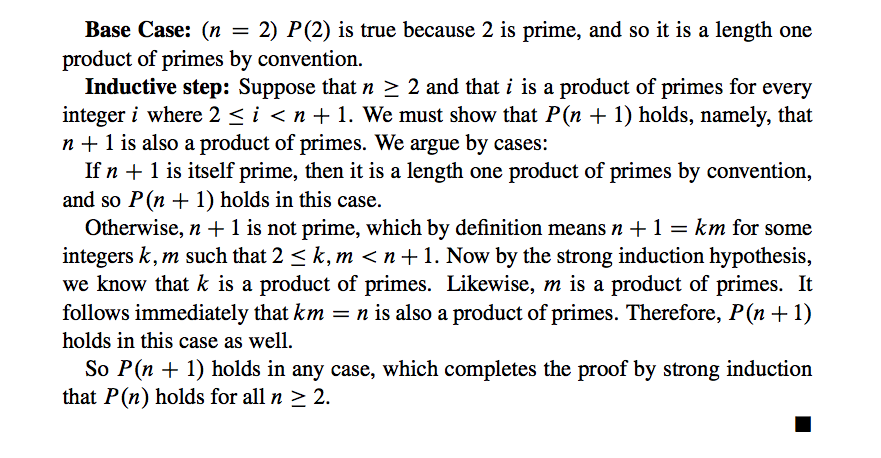
\includegraphics{images/L13/strongproof.png}
 \caption{Proof}
 \end{figure}
 
     \subsection{Strong Induction}\label{strong-induction}
 
 \begin{figure}
 \centering
 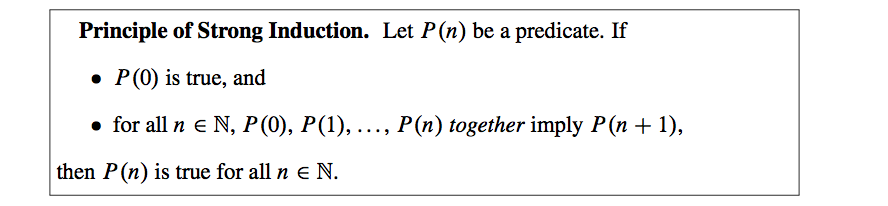
\includegraphics{images/L13/strong.png}
 \caption{Strong PMI}
 \end{figure}
 
     \subsection{Question: Another Example of Strong
 Induction}\label{question-another-example-of-strong-induction}
 
 \textbf{Question}: The country Inductia, whose unit of currency is the
 Strong, has coins worth 3Sg (3 Strongs) and 5Sg.
 
 For which amounts \(n\) of Strongs can the Inductians produce exact
 change?
 
 \begin{itemize}
 \item For all $n \geq 6,$
 \item For all $n \geq 8,$
 \item For all $n \geq 8,$ except multiples of $22$.
 \item There are infinitely many $n$ for which they cannot produe change.
 \end{itemize}
 
     \subsection{Another Example of Strong
 Induction}\label{another-example-of-strong-induction}
 
 \textbf{Question}: The country Inductia, whose unit of currency is the
 Strong, has coins worth 3Sg (3 Strongs) and 5Sg. Prove that the
 Inductians can collect coins to make change for any number that is at
 least 8 Strongs.
 
 \textbf{Proof} by strong induction
 
     \subsection{Different Ways of Changing the Inductive
 Hypothesis}\label{different-ways-of-changing-the-inductive-hypothesis}
 
 \begin{itemize}
 \tightlist
 \item
   Making the inductive hypothesis stronger has pros/cons:
 
   \begin{itemize}
   \tightlist
   \item
     PRO: stronger assumption you can rely on
   \item
     CON: need to show something stronger
   \end{itemize}
 \end{itemize}
 
     \textbf{NOTE}: Sometimes choosing the right way to strengthen the
 hypothesis is crucial to solve a problem.
 
     \subsection{Example: Tromino Tiling}\label{example-tromino-tiling}
 
 A tiling board with a special square, marked B:
 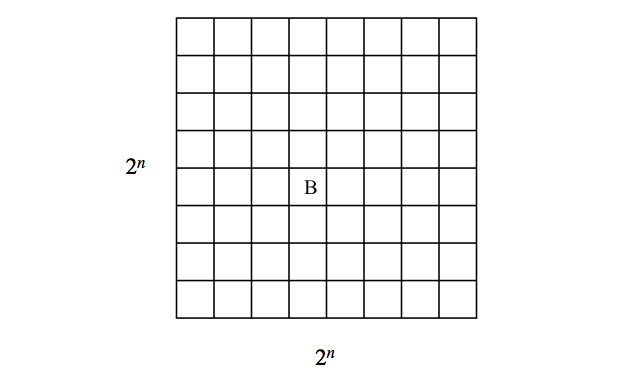
\includegraphics{images/L13/tilingb.png}
 
     A tromino: 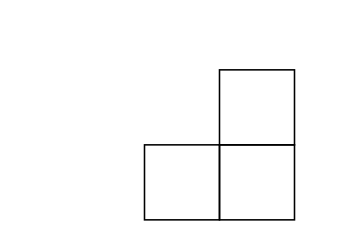
\includegraphics{images/L13/tromino.png}
 
     \textbf{Question}: can you tile the board with trominoes, leaving out
 the special square?
 
     \subsection{Tromino Tiling}\label{tromino-tiling}
 
 You are encouraged to check out the applet at the following website:
 http://www.cut-the-knot.org/Curriculum/Geometry/Tromino.shtml This may
 require you to enable Java on your browser.
 
 
     % Add a bibliography block to the postdoc
     
     
     
     \end{document}
 